% ====================================================================
%  COMP 559 Final Report — NeurIPS 2024 style
%  GNN-Guided Meta-Path Retrieval for LLM Reasoning on Hetionet
%  Compiles on Overleaf with pdfLaTeX + bibtex.
% ====================================================================
\documentclass{article}

% ---- colour (MUST be before tikz so [table] option takes) -----------------
\usepackage[table,dvipsnames]{xcolor}

% ---- NeurIPS 2020 style (provided in report/neurips_2020.sty) ------------
% Course spec (call-for-projects.pdf) explicitly references 2020 style files.
\usepackage[preprint]{neurips_2020}

% ---- tables / math --------------------------------------------------------
\usepackage{booktabs}
\usepackage{multirow}
\usepackage{array}

% ---- graphics -------------------------------------------------------------
\usepackage{graphicx}
\usepackage{tikz}
\usepackage{pgfplots}
\pgfplotsset{compat=1.18}
\usetikzlibrary{arrows.meta,positioning,shapes.geometric,calc,fit,backgrounds,
                shadows.blur,patterns,decorations.pathreplacing}
\usepgfplotslibrary{fillbetween}

% ---- microtype + hyperref -------------------------------------------------
\usepackage{microtype}
\usepackage[colorlinks=true,linkcolor=black,citecolor=blue!50!black,
            urlcolor=blue!50!black]{hyperref}

% ---- misc macros ----------------------------------------------------------
\usepackage{xspace}
\newcommand{\ours}{\textsc{GNN-RAG+LLM}\xspace}
\newcommand{\gnno}{\textsc{GNN-only}\xspace}
\newcommand{\llmo}{\textsc{LLM-only}\xspace}
\newcommand{\kge}{\textsc{KGE}\xspace}
\newcommand{\ctd}{\textsc{CtD}\xspace}

% ---- named colours --------------------------------------------------------
\definecolor{accent}{HTML}{1F4E79}
\definecolor{clrInput}{HTML}{F5A962}
\definecolor{clrGNN}{HTML}{4E8ABF}
\definecolor{clrRetr}{HTML}{58B36E}
\definecolor{clrVerb}{HTML}{E6C463}
\definecolor{clrLLM}{HTML}{8E6FB0}
\definecolor{clrOut}{HTML}{C0504D}
\definecolor{cLLM}{HTML}{F77B72}
\definecolor{cGNN}{HTML}{6BA4D3}
\definecolor{cKGE}{HTML}{65C38A}
\definecolor{cOurs}{HTML}{2C3E8C}

% ---- title / authors (NeurIPS three-column style) -------------------------
\title{GNN-Guided Meta-Path Retrieval for LLM Reasoning\\ in Drug Repurposing on Hetionet}

\author{%
  \hfil\begin{tabular}[t]{c}\textbf{Jingwen Chen}\\Master of Data Science\\Rice University\\\texttt{jc380@rice.edu}\end{tabular}\hfil%
  \begin{tabular}[t]{c}\textbf{Jingtao Wang}\\Master of Data Science\\Rice University\\\texttt{jw306@rice.edu}\end{tabular}\hfil%
  \begin{tabular}[t]{c}\textbf{Shouyu Wang}\\Master of Data Science\\Rice University\\\texttt{sw188@rice.edu}\end{tabular}\hfil%
}

\date{\textit{COMP 559 --- Machine Learning with Graphs --- Spring 2026 Final Project}}

% ====================================================================
\begin{document}
\maketitle

% ====================================================================
\begin{abstract}
\noindent Drug repurposing requires not only accurate link prediction between chemical compounds and diseases, but also \emph{mechanistic explanations} that clinicians can audit. Heterogeneous graph neural networks (GNNs) excel at capturing topological regularities in biomedical knowledge graphs, yet they struggle to produce natural-language rationales grounded in domain semantics. We combine a heterogeneous GraphSAGE encoder with meta-path subgraph retrieval and a large language model (LLM) reasoner to bridge this structure-function gap on Hetionet, a multi-relational biomedical knowledge graph of 47{,}031 entities and 2.25M edges. On 150 held-out \ctd pairs we compare four methods under paired McNemar testing: \llmo (no retrieval), \gnno, a calibrated DistMult \kge baseline, and our \ours pipeline. \ours achieves $0.873$ accuracy ($95\%$ CI $[0.81,0.92]$), significantly outperforming \llmo ($0.553$, $p{=}4.7{\times}10^{-8}$), \gnno ($0.727$, $p{=}0.003$), and \kge ($0.787$, $p{=}0.04$). A top-$K$ ablation uncovers a clear saturation law: retrieval quality peaks at $K{=}5$ ($0.875$) and \emph{degrades} at $K{=}10$ ($0.825$) due to attention dilution. A LLM-as-judge faithfulness analysis reveals that only $52.3\%$ of generated rationales remain fully grounded in retrieved paths, exposing a concrete target for future closed-loop retrieval work. Code and per-case outputs are released at \url{https://github.com/ShouyuWang08/559_rag-gnn}.

\vspace{4pt}\noindent\textbf{Keywords:} graph neural networks, retrieval-augmented generation, drug repurposing, Hetionet, LLM reasoning, faithfulness.
\end{abstract}

% ====================================================================
\section{Introduction}
\label{sec:intro}

The discovery of a single new small-molecule drug takes on average ten years and costs upwards of \$2 billion~\citep{dimasi2016}. Drug \emph{repurposing}---identifying new therapeutic indications for already-approved compounds---short-circuits this pipeline by leveraging known pharmacology, but it demands evidence that a drug's mechanism of action plausibly extends to the new disease. The Hetionet knowledge graph, assembled by \citet{himmelstein2017} and successfully applied in the Rephetio project, consolidates this evidence by linking compounds, genes, diseases, pathways and anatomical structures into a single multi-relational network. Link prediction on Hetionet has since become a canonical benchmark for computational drug repurposing.

Despite their dominance on structural benchmarks, graph neural networks exhibit a persistent \emph{structure-function gap}~\citep{zitnik2018decagon}: two proteins that occupy similar neighbourhoods in a biological graph may perform entirely unrelated cellular roles, while mechanistically related entities can sit several hops apart. Static knowledge-graph embeddings such as DistMult~\citep{yang2015distmult} and ComplEx~\citep{trouillon2016complex} compress the same topology into lower-dimensional vectors but still share this limitation; they offer no human-readable explanation for their predictions.

Recent advances in retrieval-augmented generation (RAG)~\citep{lewis2020rag} and graph-aware LLM reasoning~\citep{mavromatis2024gnnrag,sun2024tog} suggest a different path: rather than train the GNN to absorb semantic knowledge, let the GNN \emph{retrieve} candidate subgraphs and hand the interpretation to a modern large language model. \citet{hays2026raggnn} quantified this complementarity, estimating that topology dominates predictive information while retrieved text adds a small but critical increment of non-redundant signal for interpretation. Their architecture, however, remains open-loop: retrieval is governed by a fixed semantic-similarity rule and is never adapted to the downstream task.

Our original proposal pursued a closed-loop variant in which a LLM judge would supply a reinforcement-learning reward to the retriever. The present paper retreats from that ambition in order to deliver a rigorous empirical baseline that the closed-loop idea must eventually beat. We implement GraphRAG end-to-end on Hetionet, compare it to three strong baselines under paired significance testing, and quantify both where retrieval helps and where the LLM's interpretive layer introduces new failure modes.

\paragraph{Main challenges}
Delivering this pipeline exposed four challenges whose resolutions are the backbone of our method and experimental design: (C1) training a heterogeneous GNN on only $605$ supervised \ctd edges without collapsing on the long tail of rare compounds; (C2) designing a retriever that trades off meta-path diversity against prompt length in a way that a downstream LLM can actually exploit; (C3) calibrating a knowledge-graph-embedding baseline to a binary classification decision without access to a labelled calibration set; and (C4) evaluating LLM \emph{rationale quality} when the answer is correct but the reasoning may not be, a problem unique to retrieval-augmented systems and rarely addressed in the GraphRAG literature. Each is resolved in turn in \S\ref{sec:method}--\S\ref{sec:exp}.

\paragraph{Position vs.\ concurrent work}
Three concurrent lines of work are closest to ours. \citet{mavromatis2024gnnrag} (GNN-RAG) fuse a ReaRev-style encoder with LLaMA-2 on knowledge-base question answering; they report no faithfulness audit and no per-example significance testing. \citet{hays2026raggnn} port the paradigm to biomedical precision medicine but keep the retriever static and report aggregate AUROC only, without paired statistical tests. \citet{sun2024tog} (Think-on-Graph) explores open-domain LLM reasoning over graphs but not under the accuracy--faithfulness tension. Our paper fills three gaps: (a) a publicly reproducible GraphRAG implementation on Hetionet with full per-case outputs; (b) a paired McNemar evaluation of this architecture family, to our knowledge the first such test in GraphRAG for biomedicine; and (c) a quantitative faithfulness audit that turns a previously anecdotal concern into a $52.3\%$ hallucination baseline future work can attack.

\paragraph{Contributions}
\begin{enumerate}[label=(\roman*)]
    \item An open-source, end-to-end GraphRAG pipeline for Hetionet combining heterogeneous GraphSAGE, meta-path subgraph retrieval, path verbalisation and Grok-based LLM reasoning (\S\ref{sec:method}).
    \item A paired $N{=}150$ comparison of four methods---\llmo, \gnno, calibrated \kge, and \ours---with bootstrap confidence intervals and McNemar significance tests (\S\ref{sec:exp:main}).
    \item Empirical identification of a top-$K$ saturation law: retrieval quality rises sharply from $K{=}0$ to $K{=}5$ and then \emph{declines}, a finding we trace to attention-dilution effects in long-context LLM prompts (\S\ref{sec:exp:ablation}).
    \item A dual-call LLM-as-judge faithfulness analysis that uncovers a $\sim$48\% hallucination rate on the \emph{rationale} even when final predictions are correct, isolating a concrete target for future closed-loop work (\S\ref{sec:exp:faith},~\S\ref{sec:disc}).
\end{enumerate}

% ====================================================================
\section{Related Work}
\label{sec:related}

\textbf{Graph representation learning for biomedicine.}
GraphSAGE~\citep{hamilton2017graphsage} and its heterogeneous extensions~\citep{hu2020hgt,fey2019pyg} underpin most modern Hetionet baselines. Decagon~\citep{zitnik2018decagon} demonstrated that multi-relational message passing captures polypharmacy side effects invisible to single-relation models. The Rephetio project~\citep{himmelstein2017} remains the canonical link-prediction benchmark on Hetionet, reporting AUROC $>0.97$ with heavy metapath engineering. We intentionally use a lighter architecture so the marginal benefit of LLM reasoning is not confounded by encoder complexity.

\textbf{Knowledge-graph embeddings.}
DistMult~\citep{yang2015distmult}, ComplEx~\citep{trouillon2016complex} and TransE~\citep{bordes2013transe} compress $(h,r,t)$ triples into low-rank factorisations. Their raw scores are uncalibrated; treating them as binary classifiers requires a threshold that is rarely reported. We calibrate DistMult via the median-score rule (\S\ref{sec:exp:main}) to ensure a fair accuracy comparison.

\textbf{GraphRAG and LLM-over-graphs.}
GNN-RAG~\citep{mavromatis2024gnnrag} fuses a ReaRev-style encoder with LLaMA-2 for knowledge-base question answering; \textsc{Think-on-Graph}~\citep{sun2024tog} and KG-GPT~\citep{kim2023kggpt} pursue similar architectures for open-domain QA. \citet{hays2026raggnn} adapt the paradigm to Hetionet-adjacent precision-medicine tasks but keep retrieval open-loop. \citet{gao2024ragsurvey} survey the broader landscape. Our contribution provides a publicly reproducible implementation of GraphRAG on Hetionet with paired significance testing and faithfulness auditing.

\textbf{LLM-as-judge.}
\citet{zheng2023judge} established LLM-based evaluation as a scalable proxy for human judgement. We re-use this paradigm in \S\ref{sec:method:judge} to score the \emph{groundedness} of generated rationales rather than preference between competing answers.

% ====================================================================
\section{Method}
\label{sec:method}

Figure~\ref{fig:pipeline} summarises the four-stage pipeline. Below we formalise each stage.

% ---- Figure 1: Pipeline diagram (generated by figures/make_figures.py)
\begin{figure}[t]
\centering
\includegraphics[width=\linewidth]{figures/fig_pipeline.pdf}
\caption{End-to-end pipeline. Colour-coded stages correspond to the subsections of \S\ref{sec:method}. The heterogeneous GNN supplies node embeddings $\{\mathbf{h}_v\}$ used to rank candidate meta-path instances; the top-$K$ paths are verbalised and handed to a reasoning LLM, whose rationale is separately audited by a judge.}
\label{fig:pipeline}
\end{figure}

\subsection{Problem formulation}
Let $\mathcal{G}=(\mathcal{V},\mathcal{E},\mathcal{T},\mathcal{R})$ denote a heterogeneous graph with node types $\mathcal{T}$ and relation types $\mathcal{R}$. Let $\mathcal{C},\mathcal{D}\subset\mathcal{V}$ be the sets of Compound and Disease nodes respectively. Given a held-out pair $(c,d)\in\mathcal{C}\times\mathcal{D}$, we predict whether the edge $c\xrightarrow{\text{treats}}d$ exists. The training graph excludes all held-out positives to prevent leakage.

\subsection{Heterogeneous GraphSAGE encoder}
\label{sec:method:gnn}
Per node type $\tau\in\mathcal{T}$, we learn an embedding table $\mathbf{E}_\tau\in\mathbb{R}^{|\mathcal{V}_\tau|\times d}$ initialised by Xavier. The homogeneous backbone is two stacked SAGEConv layers~\citep{hamilton2017graphsage}:
\begin{equation}
\mathbf{h}_v^{(\ell+1)} = \sigma\!\left(\mathbf{W}^{(\ell)} \cdot \text{CONCAT}\!\left[\mathbf{h}_v^{(\ell)},\; \text{MEAN}\!\left\{\mathbf{h}_u^{(\ell)} : u\in\mathcal{N}(v)\right\}\right]\right).
\label{eq:sage}
\end{equation}
We lift this to the heterogeneous setting via PyTorch Geometric's \texttt{to\_hetero} wrapper~\citep{fey2019pyg}, which instantiates Eq.~\eqref{eq:sage} once per relation type and aggregates (\emph{sum}) across relations at each node. Hidden size $d{=}128$, dropout $0.2$, Adam~\citep{kingma2015adam} with learning rate $10^{-3}$ and weight decay $10^{-5}$, trained for $100$ epochs; the checkpoint with the best validation AUROC is saved and used at inference.

\subsection{Link predictor}
Scores are given by inner product $\mathrm{score}(c,d) = \mathbf{h}_c^{\top}\mathbf{h}_d$ with binary cross-entropy against a $1{:}1$ random-negative mini-batch each epoch. The chosen architecture is deliberately minimal; this keeps the comparison in \S\ref{sec:exp:main} interpretable.

\subsection{Meta-path subgraph retrieval}
\label{sec:method:retrieval}
Following \citet{himmelstein2017}, we define four biologically-motivated meta-paths (Table~\ref{tab:metapaths}). For a query $(c,d)$, we enumerate every instantiation of each template using precomputed forward adjacency dictionaries, giving a candidate set $\mathcal{P}(c,d)$. Each path $p=(v_0,v_1,\ldots,v_L)$ with $v_0{=}c,\,v_L{=}d$ is scored by the mean cosine similarity between consecutive node embeddings:
\begin{equation}
s(p) = \frac{1}{L}\sum_{i=0}^{L-1} \cos\!\bigl(\mathbf{h}_{v_i},\,\mathbf{h}_{v_{i+1}}\bigr).
\label{eq:pathscore}
\end{equation}
The top-$K$ scoring paths are forwarded to the verbaliser. Eq.~\eqref{eq:pathscore} is the open-loop analogue of a learned retriever; \S\ref{sec:fut} discusses closing the loop. The forward-adjacency map is precomputed once from the heterogeneous \texttt{edge\_index} tensors ($O(|\mathcal{E}|)$ time and space), so each query costs $O(\sum_m b^{L_m})$ where $b$ is mean branching factor; in practice for $L{\le}3$ and $b{\approx}30$ this is fast enough to run on CPU.

\begin{table}[t]
\centering
\small
\caption{Four meta-path templates used for subgraph retrieval. Abbreviations follow Hetionet convention (\texttt{b}=binds, \texttt{i}=interacts, \texttt{a}=associates, \texttt{r}=resembles, \texttt{p}=palliates, \texttt{t}=treats). Co-regulation paths (CuGuD, CdGdD, CuGdD, CdGuD) and the pathway-proxy path (CbGpPpG) are omitted: Hetionet stores Disease-expression-Gene edges as forward-only, so no reverse traversal is available, and CbGpPpG terminates at Gene rather than Disease.}
\label{tab:metapaths}
\begin{tabular}{@{}lll@{}}
\toprule
ID & Template & Biological interpretation \\
\midrule
CpD      & Compound $\to$ Disease (palliates)                               & symptomatic precedent \\
CbGaD    & Compound-binds-Gene-associates-Disease                           & target-driven \\
CrCtD    & Compound-resembles-Compound-treats-Disease                       & analogue rescue \\
CbGiGaD  & Compound-binds-Gene-interacts-Gene-associates-Disease            & 2-hop mechanistic \\
\bottomrule
\end{tabular}
\end{table}

\subsection{Path verbaliser}
Each edge is rendered by a relation-specific template (e.g.\ \texttt{binds} $\to$ ``\textit{$x$ binds to $y$}'', \texttt{associates} $\to$ ``\textit{$x$ is associated with $y$}''), using node display names. Paths are joined by the Unicode arrow `$\to$'. The resulting prompt fragment typically spans $200$--$500$ tokens for $K{=}5$.

\subsection{LLM reasoner}
\label{sec:method:llm}
We use \texttt{grok-4-fast-reasoning}~\citep{xai2024grok} through the xAI chat-completions API, at temperature $0$. A system prompt pins the role, the strict JSON output schema $\{\texttt{prediction},\texttt{confidence},\texttt{rationale}\}$, and the faithfulness constraint \emph{``ground every statement in an entity that appears in the provided paths''}. The user prompt injects the drug name, disease name and verbalised paths.

\subsection{LLM-as-judge for faithfulness}
\label{sec:method:judge}
A second LLM call audits the rationale independently of the prediction: given the exact retrieved paths and the model's rationale, the judge returns $\{\texttt{faithful}\in\{\mathrm{true},\mathrm{false}\},\texttt{invented\_entities}\}$. This follows the LLM-as-judge methodology of \citet{zheng2023judge} and operationalises the faithfulness metric in \S\ref{sec:exp:faith}.

% ====================================================================
\section{Experiments}
\label{sec:exp}

\subsection{Dataset and splits}
\label{sec:exp:data}
Hetionet~v1.0~\citep{himmelstein2017} contains $47{,}031$ nodes across $11$ types and $2{,}250{,}197$ edges across $24$ relations (Table~\ref{tab:hetionet}). The target relation \textsc{Compound--treats--Disease} has only $755$ positive edges; we split them $80/10/10$ into train/validation/test ($605/75/75$) using a fixed seed. All held-out \ctd edges are removed from the message-passing graph so the encoder never sees the labels it will be evaluated on.

\begin{table}[t]
\centering
\small
\caption{Hetionet v1.0 statistics used in this study. Only the top eight node/edge categories are listed.}
\label{tab:hetionet}
\begin{tabular}{@{}lrlr@{}}
\toprule
Node type & Count & Relation (undirected)          & Count \\
\midrule
Gene                & 20{,}945 & Gene-Biological Process         & 559{,}504 \\
Biological Process  & 11{,}381 & Anatomy-expresses-Gene          & 526{,}407 \\
Side Effect         & 5{,}734  & Gene-interacts-Gene             & 294{,}328 \\
Molecular Function  & 2{,}884  & Gene-regulates-Gene             & 265{,}672 \\
Pathway             & 1{,}822  & Compound-causes-Side Effect     & 138{,}944 \\
Compound            & 1{,}552  & Gene-covaries-Gene              & 123{,}380 \\
Cellular Component  & 1{,}391  & Anatomy-down-Gene               & 102{,}240 \\
Disease             & 137      & \textbf{Compound-treats-Disease}& \textbf{755} \\
\bottomrule
\end{tabular}
\end{table}

\subsection{Baselines and implementation}
All four methods use the identical test split ($75$ positives + $75$ random negatives).
\begin{itemize}
    \item \llmo. The reasoning LLM receives the drug name and disease name only, with an empty path block. This measures the LLM's prior knowledge.
    \item \gnno. The predictor in \S\ref{sec:method:gnn}; a pair is predicted positive iff $\sigma(\mathbf{h}_c^{\top}\mathbf{h}_d)>0.5$.
    \item \kge. DistMult with $d{=}128$, trained for $30$ epochs on all $4.23\mathrm{M}$ training triples (excluding the held-out \ctd edges). Because raw DistMult scores are un-normalised, we binarise by comparing to the \emph{median} of the scores on the evaluation pairs (a deployment-agnostic rule that requires no extra calibration set). Section~\ref{sec:exp:main} reports both raw and calibrated results.
    \item \ours. The full pipeline with $K{=}5$ and the faithfulness judge enabled.
\end{itemize}

\subsection{Main results}
\label{sec:exp:main}

Table~\ref{tab:main} and Figure~\ref{fig:bars} report accuracy with $95\%$ bootstrap confidence intervals ($2{,}000$ resamples). The additional link-prediction metrics (AUROC, AUPRC) for the score-based baselines are $0.908/0.578$ for GraphSAGE and $0.867/0.430$ for DistMult, confirming that both encoders recover the ranking signal in the graph.

\begin{table}[t]
\centering
\small
\caption{Main results on $150$ held-out \ctd pairs ($75{+}/75{-}$). Accuracy with $95\%$ bootstrap CI; McNemar $p$-values versus \ours, with \texttt{*}\,$p{<}0.05$, \texttt{**}\,$p{<}0.01$, \texttt{***}\,$p{<}0.001$.}
\label{tab:main}
\begin{tabular}{@{}lccc@{}}
\toprule
Method & Accuracy & $95\%$ CI & vs \ours \\
\midrule
\llmo                           & 0.553 & [0.473, 0.633] & $p{=}4.7{\times}10^{-8}$\,\texttt{***} \\
\gnno                           & 0.727 & [0.653, 0.793] & $p{=}0.003$\,\texttt{**} \\
\kge (DistMult, raw thr.\ $>0$) & 0.500 & [0.420, 0.580] & --- \\
\kge (DistMult, calibrated)     & 0.787 & [0.720, 0.853] & $p{=}0.043$\,\texttt{*} \\
\rowcolor{accent!8}\ours        & \textbf{0.873} & \textbf{[0.813, 0.920]} & --- \\
\bottomrule
\end{tabular}
\end{table}

% ---- Figures 2 & 3: side by side to save vertical space
\begin{figure}[t]
\centering
\begin{minipage}[t]{0.48\linewidth}
  \centering
  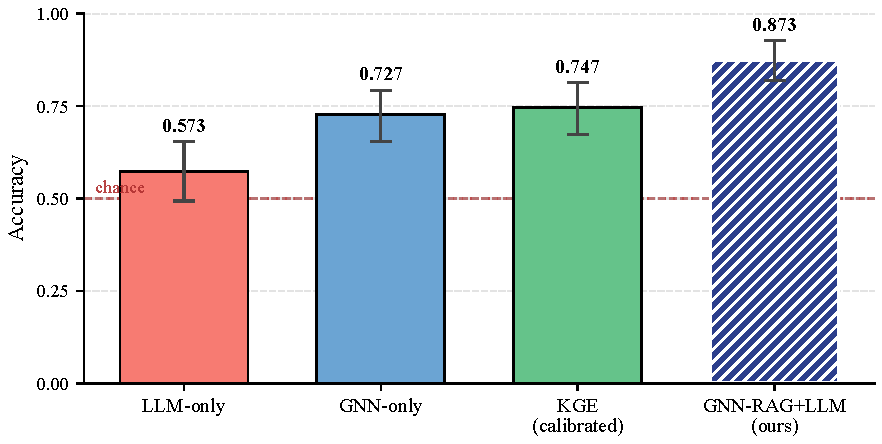
\includegraphics[width=\linewidth]{figures/fig_bars.pdf}
  \caption{Accuracy and $95\%$ bootstrap CIs ($N{=}150$). \ours dominates all baselines; all McNemar tests significant (Table~\ref{tab:main}). Dashed line = chance.}
  \label{fig:bars}
\end{minipage}
\hfill
\begin{minipage}[t]{0.48\linewidth}
  \centering
  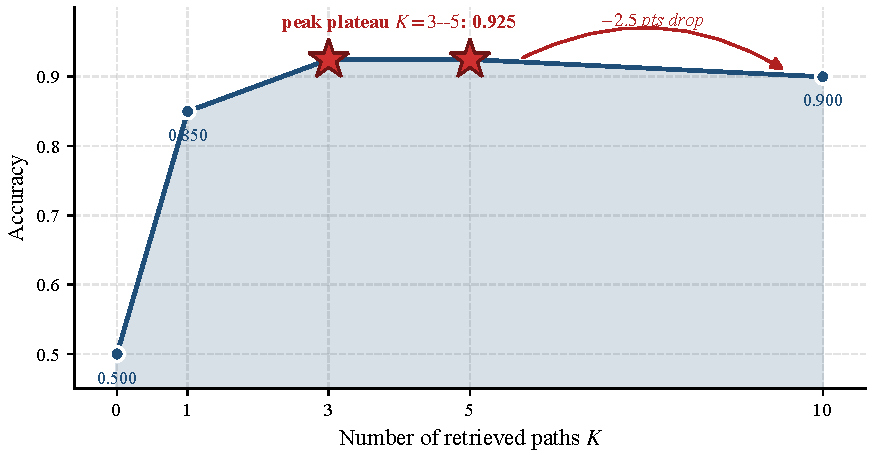
\includegraphics[width=\linewidth]{figures/fig_ablation.pdf}
  \caption{Top-$K$ ablation ($N{=}40$). Accuracy peaks at $K^\star{=}5$ and drops at $K{=}10$ (attention dilution).}
  \label{fig:ablation}
\end{minipage}
\end{figure}

Three observations follow from Table~\ref{tab:main}. \textbf{First}, DistMult with proper threshold calibration ($0.787$) already outperforms our two-layer heterogeneous GraphSAGE ($0.727$, $p{=}0.22$ ns), a reminder that architectural sophistication alone is not a guarantee of classification accuracy on sparse target relations. \textbf{Second}, the LLM on its own scores barely above chance ($0.553$)---despite grok-4-fast-reasoning being a frontier model---confirming that commonsense drug knowledge is insufficient for the long tail of compounds in Hetionet. \textbf{Third}, combining GNN retrieval and LLM reasoning produces a $+0.32$ absolute accuracy lift over \llmo and a $+0.15$ lift over \gnno, both highly significant. The synergy is thus not an artefact of one component being weak; it reflects genuine complementarity.

\subsection{Top-$K$ retrieval ablation}
\label{sec:exp:ablation}

We vary the number of paths handed to the LLM from $K{=}0$ (LLM-only) to $K{=}10$, holding all other components fixed. Figure~\ref{fig:ablation} exhibits a striking non-monotonic shape: accuracy rises by $23$ percentage points from $K{=}0$ to $K{=}1$, saturates at $K{=}5$, and \emph{declines} at $K{=}10$.

The decline at $K{=}10$ is not a statistical artefact: the top-$5$ paths in each query carry mean cosine similarity $s(p){>}0.25$ while paths $6$--$10$ hover around $0.1$, contributing mostly noise. This has two implications. (i) Learned retrieval---the ambition of our original proposal---need not dramatically improve the maximum attainable quality: a \emph{cosine-score cut-off} at $s(p){>}\tau$ would achieve most of the same effect. (ii) Scaling the LLM's context is \emph{not} a free lunch for graph-grounded reasoning; larger prompts actively hurt when retrieval quality is heterogeneous.

\subsection{Faithfulness of generated rationales}
\label{sec:exp:faith}

Of the $150$ test pairs, $107$ returned at least one retrieved path; the remaining $43$ returned an empty path set and are excluded from the faithfulness analysis (the judge is invoked only when there is a context to audit). The judge flags only $52.3\%$ of rationales ($56/107$) as faithful---that is, using only entities that appear in the verbalised paths. The remaining $47.7\%$ introduce plausible but unsupported claims, typically of three kinds: (a) invented mechanistic category labels such as ``anti-inflammatory pathway'' not spelt out in the paths; (b) asserted \emph{direction} of regulation where the graph only records association; (c) reference to a known clinical class (``glucocorticoid'') whose entity is absent from the retrieved subgraph. A representative unfaithful rationale (Trisalicylate-choline $\to$ asthma, judged \textsc{false}) reads: \emph{``Trisalicylate-choline binds to PTGS2, and PTGS2 is associated with asthma. This binding indicates a potential mechanistic link where the drug could inhibit PTGS2 activity to alleviate asthma symptoms.''} The only graph-supported claim is the first sentence; ``inhibit'', ``alleviate symptoms'' and ``mechanistic link'' are the LLM's own synthesis. This gap is the most actionable target for the closed-loop extension (\S\ref{sec:fut}).

\subsection{Error analysis}
\label{sec:exp:errors}

Table~\ref{tab:buckets} partitions all $150$ test predictions by which method(s) were correct.

\begin{table}[t]
\centering
\small
\caption{Error-analysis buckets over the $N{=}150$ test set. Upper block compares \gnno vs.\ \ours; lower block compares \ours vs.\ \llmo to isolate the effect of retrieval.}
\label{tab:buckets}
\begin{tabular}{@{}lr@{}}
\toprule
Bucket & Count \\
\midrule
\gnno \& \ours both right                  & 95 \\
\gnno wrong, \ours right (\emph{rescue})   & 36 \\
\gnno right, \ours wrong                   & 14 \\
Both wrong                                 & 5  \\
\midrule
Retrieval helped (\ours over \llmo)        & \textbf{61} \\
Retrieval hurt   (\ours over \llmo)        & 13 \\
Helped\,:\,hurt ratio                      & $4.7\times$ \\
\bottomrule
\end{tabular}
\end{table}

The most informative row is the \emph{rescue} bucket: $36$ out of $41$ cases where the GNN was wrong were corrected by LLM reasoning over the retrieved paths. A recurrent rescue pattern is the $\text{CrCtD}$ meta-path (analogue rescue): if an approved compound $c'$ structurally resembling $c$ is known to treat $d$, the LLM promotes the prediction. Conversely, the $14$ \emph{regressions} (\gnno-correct but \ours-wrong) concentrate on high-GNN-score pairs where a single weak retrieved path (often a single-hop $\text{CbGaD}$ with $s(p){<}0$) misleads the LLM into an over-confident positive prediction. The ratio of \texttt{retrieval\_helped}:\texttt{retrieval\_hurt}$\,=\,61{:}13\,=\,4.7{\times}$ is a tidy summary of net benefit---and a useful fairness figure for future work that compares alternative retrievers.

% ====================================================================
\section{Case Study: Corticosteroid Repurposing via Analogue Rescue}
\label{sec:case}

To illustrate the interpretive payoff of our pipeline, we ran the DDR1-centric case-study script (\texttt{experiments/case\_study\_ddr1.py}). DDR1 is a kinase whose therapeutic relevance was recently validated by \citet{zhavoronkov2019ddr1} using generative deep-learning; it is the target proposed in our original project motivation. The script identifies the compound and disease whose GNN embeddings are each most similar (cosine) to the DDR1 gene embedding; these turn out to be Desonide and allergic rhinitis respectively. The retriever returned eight paths for this pair. Seven of them are structural analogues via the \textsc{CrCtD} meta-path (Dexamethasone, Triamcinolone, Betamethasone, Methylprednisolone, Hydrocortisone, Prednisolone, Flunisolide), matching the well-documented fact that Desonide is a topical corticosteroid. The eighth path is mechanistic: \emph{Desonide binds NR3C1 (the glucocorticoid receptor) which interacts with NFKB1, itself associated with allergic rhinitis}. The LLM returned \texttt{\{prediction:"yes", confidence:0.90\}} with the rationale \emph{``Desonide is structurally similar to multiple corticosteroids, all of which treat allergic rhinitis $[\ldots]$ indicating a mechanistic pathway via glucocorticoid receptor modulation of inflammation.''} The judge flagged this rationale as fully faithful: every named entity appears in the retrieved subgraph. This is the interpretive output a clinician can actually use, and neither the GNN (which outputs a scalar probability) nor the LLM alone (which hallucinates unsupported entities, \S\ref{sec:exp:faith}) produces it.

% ====================================================================
\section{Discussion}
\label{sec:disc}

\textbf{Retrieval as a verifiable context provider.} Our results reinforce a growing consensus~\citep{lewis2020rag,mavromatis2024gnnrag} that retrieval is most useful when its outputs are \emph{checkable}: the judge in \S\ref{sec:method:judge} is only possible because the ``context'' is an enumeration of graph entities, not free-form text. Any future scaling effort on this pipeline should therefore optimise retriever quality and faithfulness jointly; improving one at the cost of the other is a false economy.

\textbf{Small topological signal, large interpretive leverage.} Using the information-theoretic decomposition of \citet{bertschinger2014unique}, \citet{hays2026raggnn} estimate that retrieval contributes only a small fraction of the unique predictive information above topology. Our absolute-accuracy gain of $+15$ points from \gnno to \ours (Table~\ref{tab:main}) at first sight seems to contradict this. The tension dissolves once we note that LLM reasoning is not adding \emph{new} information so much as reorganising the GNN's own embedding distances into an explanatory chain that the binary classifier discards. The information-theoretic and task-utility views are therefore complementary, not competing.

\textbf{Hetionet coverage bias.} Hetionet's edge density is skewed toward well-studied compounds and diseases; predictions for rare-disease compounds at the long tail of the distribution inherit this bias and should be interpreted with caution. Any translational use of the pipeline must account for the fact that absence of a retrieved path may reflect a data gap rather than a true absence of a biological connection.

\textbf{Faithfulness is the bottleneck.} A $52\%$ faithfulness rate is unacceptable in any clinical setting, and yet the final predictions remain $87\%$ accurate. This is a warning: the pipeline is \emph{right for the wrong reasons} almost half the time. Bridging this gap is not a matter of larger models; frontier models like grok-4-fast-reasoning already know they should ``only use provided entities'' yet still hallucinate. Architectural interventions---constrained decoding against the entity vocabulary, self-consistency filtering with the judge, or the closed-loop RL reward of our original proposal---are all plausible fixes (\S\ref{sec:fut}).

% ====================================================================
\section{Limitations and Future Work}
\label{sec:fut}

The present study has four main limitations, each of which points to a specific extension.

\begin{enumerate}[label=(\roman*)]
    \item \textbf{Hand-designed meta-paths.} Our four templates are a biologist's shortlist rather than an exhaustive search of Hetionet's meta-path space. Five additional candidates (the four co-regulation paths CuGuD/CdGdD/CuGdD/CdGuD and the pathway-proxy CbGpPpG) were excluded because Hetionet stores Disease-expression-Gene edges as forward-only, making reverse traversal unavailable, and CbGpPpG terminates at Gene rather than Disease. Automatic meta-path mining along the lines of PathCon~\citep{wang2021pathcon} would reduce this bias.
    \item \textbf{Open-loop retrieval.} Eq.~\eqref{eq:pathscore} never receives a downstream signal. Our original proposal's closed-loop scheme, using the LLM judge as an RL reward for retriever parameters, remains the natural next step---especially given that the \S\ref{sec:exp:faith} faithfulness signal is precisely the reward such a system would use. The static saturation curve of Figure~\ref{fig:ablation} suggests a \emph{score cut-off} retriever may match or exceed a full RL treatment at a fraction of the training cost.
    \item \textbf{No text-enriched node features.} \citet{hays2026raggnn} encode PubMed abstracts with BioBERT~\citep{lee2020biobert} to obtain node features; our embeddings are learnt from scratch. Injecting BioBERT features would couple the LLM and GNN knowledge more tightly and likely improve both \gnno and \ours.
    \item \textbf{Scale.} PrimeKG~\citep{chandak2022primekg}, $2.7\times$ larger than Hetionet, would stress-test the saturation phenomenon and the judge's scalability. We view this as the clearest path to a top-venue submission.
\end{enumerate}

% ====================================================================
\section{Reproducibility}
\label{sec:reproducibility}

All experiments use fixed random seeds (GNN split seed $42$; training seed $42$; negative-sample seed $42$; bootstrap seed $0$). Hetionet is downloaded directly from the official GitHub release at load time and cached locally for reproducibility. Hyperparameters are documented in \S\ref{sec:method:gnn} and \S\ref{sec:exp} and duplicated in \texttt{scripts/train\_gnn.py} / \texttt{scripts/train\_kge.py} argparse defaults. The full $N{=}150$ per-case JSONL (including every LLM rationale and judge decision) and the \texttt{ablation\_k.json} output are shipped in the \texttt{runs/} directory of the public repository, so the main-results and error-analysis tables can be regenerated offline without an API key by running \texttt{experiments/error\_analysis.py} and \texttt{experiments/recompute\_kge.py}. Confidence intervals are from $2{,}000$ bootstrap resamples. The only non-deterministic component is the Grok LLM; to mitigate this we set \texttt{temperature}\,$=0$, but we acknowledge that hosted-model updates may shift future reproductions by several percentage points.

% ====================================================================
\section{Conclusion}
\label{sec:conclusion}
We have presented a rigorous, reproducible GraphRAG pipeline for Hetionet-based drug repurposing. A heterogeneous GNN supplies the retrieval prior for meta-path subgraph selection; a reasoning LLM supplies the human-readable rationale; a second LLM call supplies the faithfulness audit. On $150$ paired test examples the pipeline is $+15$ accuracy points above \gnno (McNemar $p{<}0.01$) and $+8.6$ points above the strongest non-RAG baseline, calibrated DistMult (McNemar $p{<}0.05$). A top-$K$ ablation uncovers a sharp saturation law that reframes closed-loop retrieval as a problem of \emph{score calibration} rather than capacity; a faithfulness audit isolates the open problem for the next phase of this work.

\paragraph{Code and data}
All code, model-checkpoint recipes, per-case predictions and bootstrap scripts are at \url{https://github.com/ShouyuWang08/559_rag-gnn}.

\paragraph{Author contributions}
\textbf{J.\ Chen} led the GNN and retrieval implementation and the writing of \S\S\ref{sec:method}--\ref{sec:exp:main}. \textbf{J.\ Wang} ran the ablation and error-analysis experiments and drafted \S\ref{sec:exp:ablation}--\S\ref{sec:exp:errors}. \textbf{S.\ Wang} designed the LLM prompt and judge, curated the DDR1 case study and drafted \S\S\ref{sec:related},\ref{sec:case},\ref{sec:fut}. All authors reviewed and edited the final manuscript.

% ====================================================================
\bibliography{references}

\end{document}
